\chapter{Análisis}

\section{Funcionamiento del algoritmo}

% Explicación del algoritmo a nivel conceptual basándose en el libro de referencia de Birge.

El primer paso imprescindible para la realización de este proyecto será entender el algoritmo con el que se trabajará. Se debe estudiar el funcionamiento teórico de la Programación Estocástica y el algoritmo Progressive Hedging con el objetivo de entender posteriormente su implementación en PySP. \\

Como referencia principal se utiliza el libro {\it Introduction to Stochastic Programming} \cite{stochasticProgramming}. Como se explicó anteriormente, la programación estocástica resuelve problemas donde existe un cierto nivel de incertidumbre. A lo largo de esta fase de análisis utilizaremos el ejemplo ``Farmer'' para ver un problema real en funcionamiento que sea sencillo de entender. Este problema está explicado en el libro anterior e incluido como ejemplo en el repositorio de Pyomo por lo que será una referencia muy útil.\\

En el problema del granjero, nos encontramos con una superficie concreta donde podemos plantar 3 tipos diferentes de cultivos. El problema de optimización es especificar la cantidad de superficie óptima para cada uno de los cultivos. Para llegar a la solución óptima se deben tener en cuenta múltiples restricciones como el precio por tonelada de cada cultivo, la cantidad de cultivo que conseguimos por unidad de superficie, su coste o cantidad mínima necesaria para venderlo. La incertidumbre en este problema viene dada por la eficiencia de cada cultivo. Aunque plantemos una cantidad concreta en una superficie específica, no podemos asegurar la cantidad de producto que conseguiremos pues depende de multitud de factores externos. Conocemos por datos pasados una aproximación de lo que producirá una cierta plantación, pero debemos considerar los escenarios en que esta producción será menor o superior. Con esto, tenemos un árbol de escenarios como el explicado en la \autoref{fig:scenario-tree}.\\

Para resolver este tipo de problemas, se utilizará el algoritmo \textit{Progressive Hedging}. Este algoritmo se ejecuta iterativamente y funciona descomponiendo el árbol de escenarios en problemas individuales. Cada rama del árbol se transforma en un problema lineal que se puede procesar directamente para obtener un resultado. Si simplemente hacemos esta descomposición y resolución, tendremos múltiples soluciones diferentes en función de los escenarios que existían en cada camino. Para poder obtener una solución correcta que tenga en cuenta todos los escenarios, debemos conseguir que todas las soluciones individuales convergan a un mismo valor (considerando un cierto margen de error). Esta convergencia se consigue iterando sobre el procesamiento de estos subproblemas. Evidentemente debemos hacer modificaciones en los mismos para poder conseguir la convergencia. Entre cada iteración se van a modificar las variables de las que depende cada subproblema siguiendo la fórmula definida por el algoritmo. El parámetro principal es la variable $\rho$, que no es específica de ningún problema. Esta variable se puede denominar como ``penalizador'' que influirá en cómo se modifican el resto de variables para hacer que sus valores tiendan a la solución buscada.

\section{Analizando Pyomo}

% Cómo desplegar el proyecto para ver como funciona. Usaremos el ejemplo Farmer visto en el punto anterior.
% Procedimiento de análisis utilizando la salida --verbose y apoyándose en los apuntes de Onenote.

Una vez entendido el funcionamiento teórico del algoritmo, procedemos a ver la implementación del mismo en Pyomo. Podemos acudir a la propia documentación de PySP para hacernos una idea inicial de su funcionamiento. En este documento \cite{local_pyspdoc} se especifica cómo ejecutar el algoritmo mediante el comando \texttt{runph}. También especifica cómo utilizar Pyro para resolver el problema de forma paralela.\\

En este punto, necesitamos desplegar el proyecto para poder verlo en funcionamiento. El entorno sobre el que trabajaremos es el siguiente:

\begin{itemize}
    \item Para trabajar con el código se ha realizado un \textit{fork} del proyecto original en GitHub.
    \item Como IDE se utilizará PyCharm sobre Fedora 27.
    \item El código funcionará sobre un entorno virtual de Python 3.6 creado específicamente para este proyecto.
\end{itemize}

El primer paso será establecer una configuración de ejecución para el ejemplo \textit{Farmer}. Pyomo incluye una opción \texttt{--verbose} que proporciona una salida muy detallada de la ejecución y será extremadamente útil para este análisis, sobre todo, analizando la ejecución con Pyro.

Pyomo define comandos concretos para la ejecución de sus distintos módulos así que debemos buscar cuál es el punto de entrada del comando \texttt{runph}. Vemos que se utiliza un lenguaje de etiquetas personalizadas \texttt{@pyomo\_command} para definir estos puntos de entrada concretos. Si queremos ejecutar estos comandos desde el IDE, debemos hacer una modificación al archivo que queramos ejecutar para hacerlo ejecutable como script. En este caso, el archivo \textit{phinit.py} es el punto de entrada del método \texttt{runph}:

\begin{figure}[H]
    \centerline{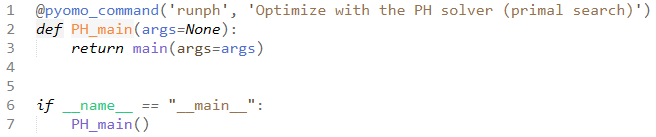
\includegraphics[width=15cm]{figuras/codigo/runph-command.png}}
\end{figure}

Con esta modificación podemos ejecutar el archivo como un script y será equivalente a ejecutar el comando \texttt{runph}. Podemos crear una configuración de ejecución en el IDE y usar la ejecución paso a paso para tener una visión general de la implementación. \\

Usando una herramienta incluida en PyCharm, podemos generar un árbol visual de llamadas a métodos. Esto genera la imagen \autoref{fig:call-tree} que representa el flujo que sigue la ejecución secuencial del algoritmo PH.

\begin{figure}[]
    \centerline{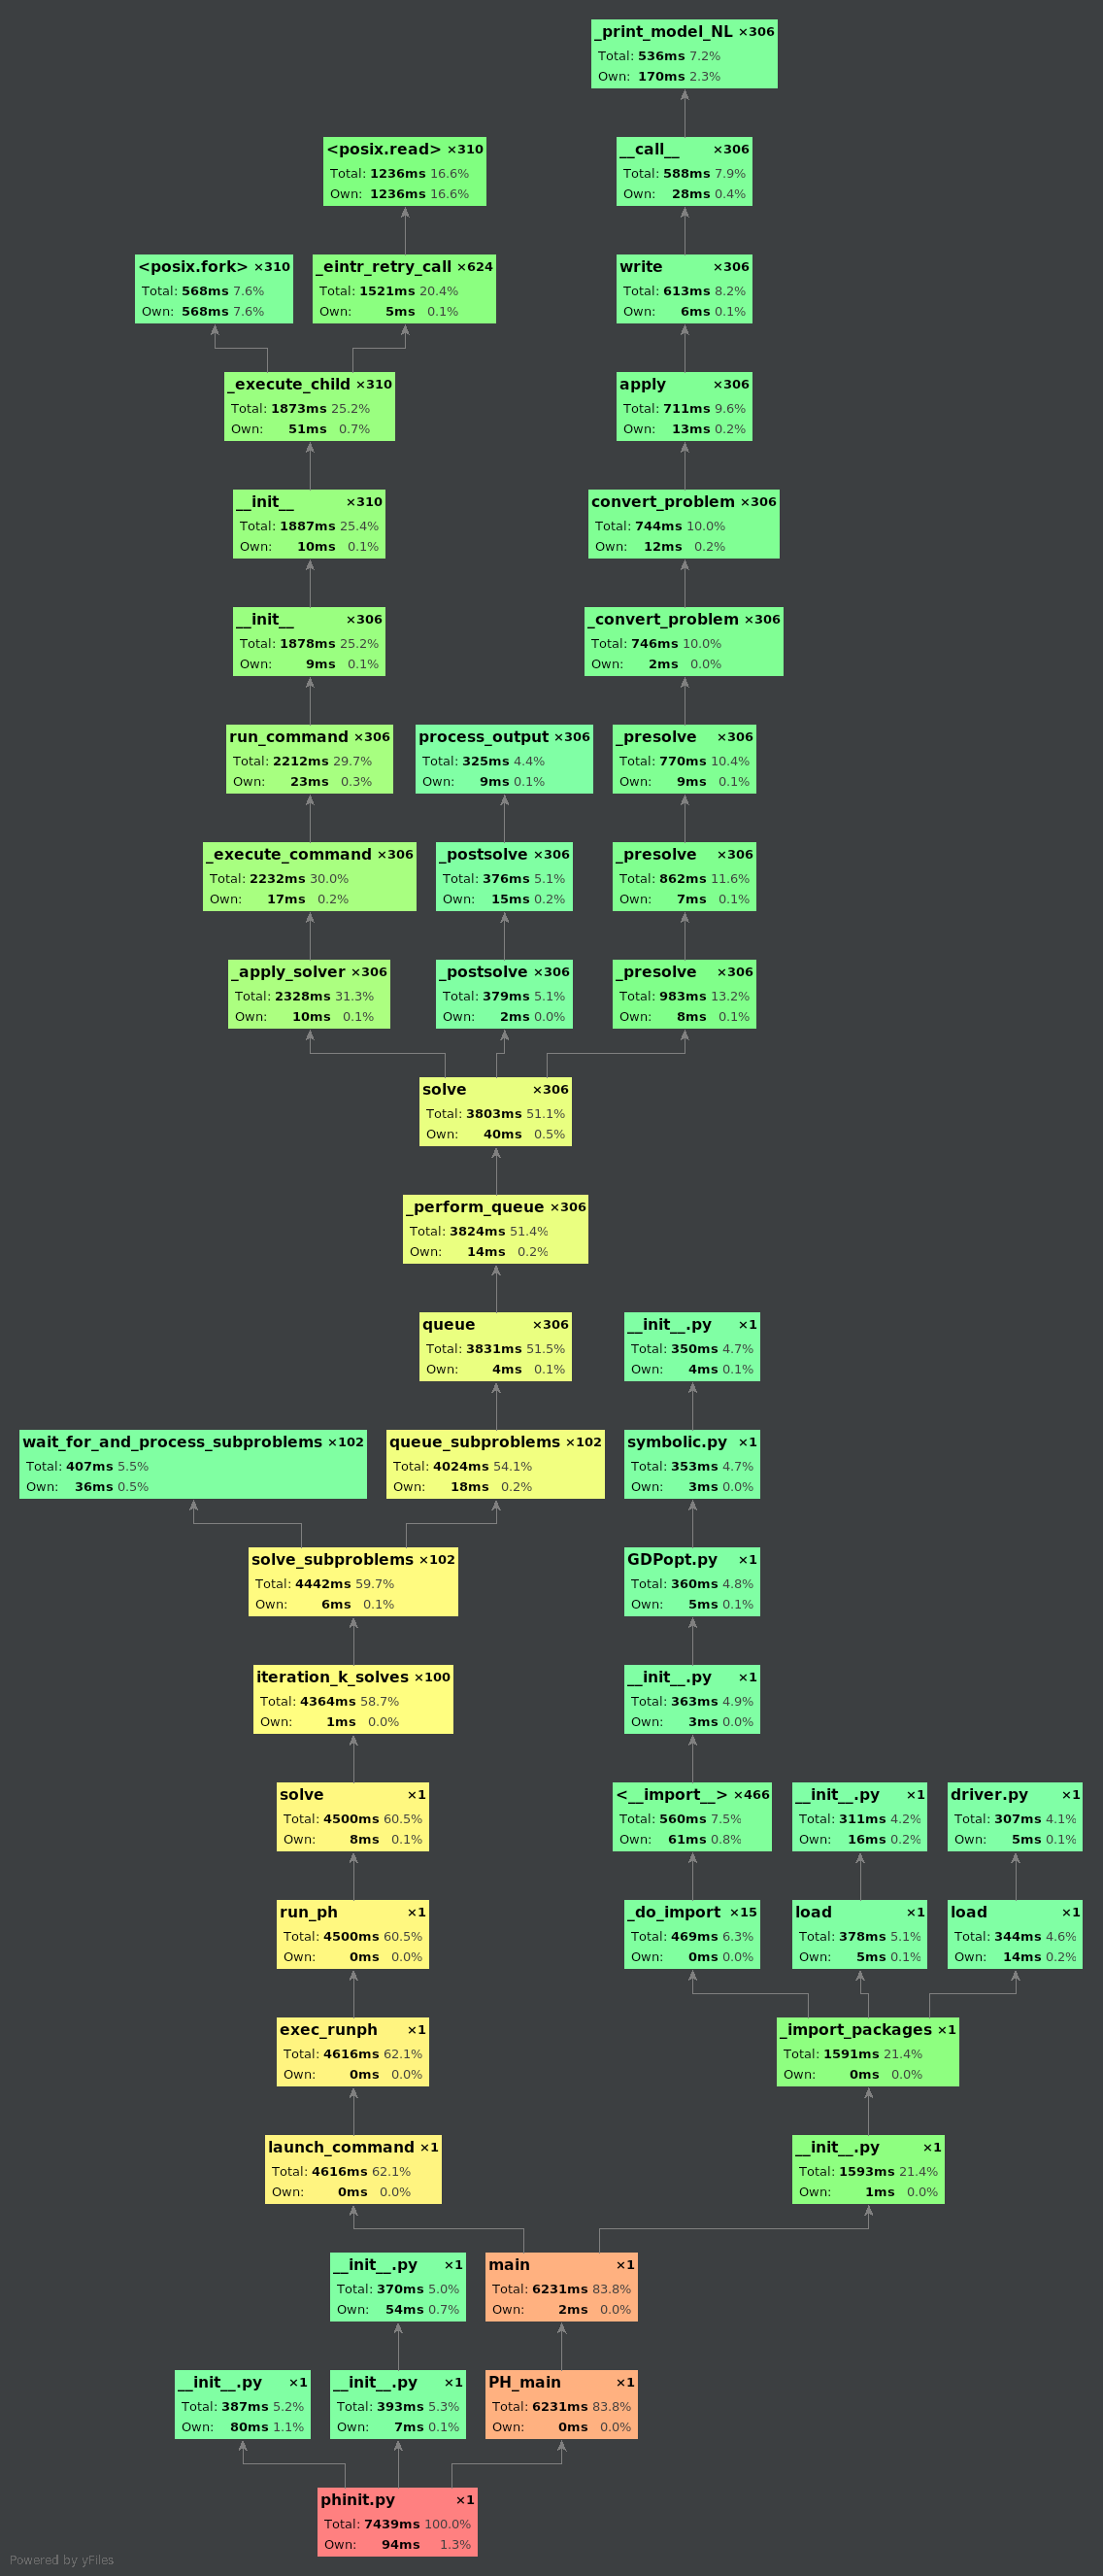
\includegraphics[width=10cm]{figuras/analisis/call-tree.png}}
    \caption{Árbol de llamadas en runph}
    \label{fig:call-tree}
\end{figure}

Podemos ignorar la rama de la derecha que se limita a la inicialización de los módulos Python. Lo relevante comienza en el método \texttt{run\_ph}. Vemos que se ejecuta el método \texttt{iteration\_k\_solves} y, aunque no está especificado en el diagrama, existe un método similar para la iteración 0, pues esta primera iteración es diferente al resto en el algoritmo PH.
En el siguiente paso observamos la primera decisión de diseño importante, se utiliza una cola para solucionar los problemas. Para cada subproblema especificado en el árbol se genera una tarea y se pone en cola. En un segundo método, se espera por los resultados. En esta ejecución secuencial esto no es muy relevante, pero lo será cuando veamos la implementación paralela.\\

En cuanto a la ejecución de la resolución, podemos distinguir tres fases: presolve, solve y postsolve:

\begin{itemize}
    \item En el \textbf{presolve} se preprocesan los escenarios del problema y se escriben en un archivo con el formato especificado. En este caso se escribe un archivo con el formato ``nl'' (\texttt{\_print\_model\_NL}) aceptado por solvers que siguen la interfaz AMPL \cite{AMPL}.
    \item En \textbf{\_apply\_solver} se utiliza el archivo generado en el paso anterior y la ruta al ejecutable del solver escogido (en nuestro caso usaremos ``minos'') para crear un comando. Esto se ejecuta como un comando en el sistema operativo y Python recoge el resultado.
    \item En el \textbf{postsolve} se procesa la salida recuperada del solver y se adapta en función del formato de salida.
\end{itemize}

En el método \texttt{solve} de \texttt{runph} es donde podemos encontrar el bucle principal que ejecuta los solves de cada iteración y realiza los cálculos necesarios para modificar los valores de cada subproblema. Al final de cada iteración se hace una prueba de convergencia que será la que indique la finalización del algoritmo.\\

Para nuestra implementación paralela analizaremos a continuación la implementación actual con Pyro. En este caso, por ser necesario lanzar múltiples procesos a la vez (el servidor de nombres, el propio \texttt{runph} y los workers), no podemos utilizar la ejecución paso a paso del IDE. En esta fase del análisis haremos usaremos la salida generada por la ejecución que, como dijimos antes, puede ser bastante específica haciendo uso de la opción \texttt{--verbose}. Analizando esta salida, podemos generar una traza con las operaciones realizadas:\\

\begin{itemize}
    \item Import model \& scenario.
    \item Construct solver manager.
    \item Construct solver.
    \item Wait for n servers to initialize.
    \item Instance each scenario.
    \item Post-instance-creation PHSolverServer plugins.
    \item Post-initialization PHSolverServer plugins.
    \item Post-initialization PH plugins.
    \item \textbf{Start PH}
    \begin{itemize}
        \item Iteration 0.
        \begin{itemize}
            \item Sync fixed variable status.
            \item Queue each solve for each scenario.
            \item Wait for scenario sub-problem solves.
            \item Pre-iteration-0-solve PHSolverServer plugins.
            \item Solve scenarios.
            \item Load all solutions.
            \item Post-iteration-0-solve PHSolverServer plugins.
            \item Convergence test.
            \item Transmitting request to activate PH objective proximal terms to PH solver servers.
            \item Transmitting request to activate PH objective weight terms to PH solver servers.
        \end{itemize}
        \item Iteration k.
        \begin{itemize}
            \item Sync fixed variable status.
            \item Transmit xbars.
            \item Transmit weights.
            \item Transmit rhos.
            \item Queue solve for each scenrio.
            \item Wait for scenario sub-problem solves.
            \item Pre-iteration-k-solve PHSolverServer plugins.
            \item Solve scenarios.
            \item Load all solutions.
            \item Post-iteration-k-solve PHSolverServer plugins.
        \end{itemize}
    \end{itemize}
\end{itemize}

En esta traza vemos la importancia que tiene el uso de una cola en la resolución de los problemas de forma paralela. El hilo principal pondrá tareas en esta cola y estas serán distribuidas a los distintos nodos de trabajo. Debemos identificar los objetos que están llevando esto a cabo. El objeto \texttt{PHSolverServer} es el encargado de ejecutar la resolución de cada subproblema y todas las tareas que se le pasen desde el hilo principal. Tendremos una instancia de este objeto por cada subproblema a resolver. En el ejemplo del \textit{Farmer}, como disponemos de 3 escenarios, tendremos tres instancias de \texttt{PHSolverServer} trabajando en paralelo. A estos obetos que realizan el trabajo en paralelo se los denominará normalmente como \textit{workers} a lo largo de este trabajo. El otro objeto relevante es el solver manager. Este objeto es el que define la distribución del trabajo. En el caso de la ejecución secuencial se utiliza \texttt{--solver-manager=serial} y, en este ejemplo, \texttt{--solver-manager=phpyro}. El solver manager se encarga de gestionar la cola de trabajos y especifica cómo se ejecutan.\\

En la traza anterior podemos observar claramente la comunicación entre el hilo principal y los workers. En cada iteración se solicita la resolución de un problema y se recoge su solución. Con esta solución se calculan las nuevas variables de control que serán retransmitidas al principio de la siguiente iteración. \\

Llegados a este punto tenemos una idea bastante concreta de la implementación del algoritmo en Pyomo. Con este conocimiento podemos comenzar el análisis de tecnologías teniendo en cuenta su posible integración y, posteriormente, comenzar con el diseño de la solución.

\section{Análisis de herramientas}

\subsection{Spark}

% Explicación más detallada de Spark, sus módulos de SQL, stream, ml, etc. 
% Cómo funcionan los RDD.

La principal opción para la implementación de este proyecto es Spark. Como se explicó anteriormente, Spark es un framework de código abierto para la programación en entornos distribuidos. Es una herramienta encuadrada en el campo del Big Data y ofrece distintos módulos de funcionamiento.\\

El módulo principal de Spark se basa en la utilización de RDDs (\textit{``Resilient Distributed Datasets''}). Un RDD es una colección de elementos particionados en los nodos del cluster en el que se ejecute Spark. Las operaciones sobre estos objetos se realizarán automáticamente en paralelo. Para trabajar con estos RDDs, Spark define transformaciones y acciones. Una transformación modifica los elementos del RDD para generar uno nuevo. Las acciones procesan el RDD para devolver un resultado concreto. Esta diferencia es clave para entender el funcionamiento de Spark. Spark hace uso de la evaluación perezosa para las transformaciones, es decir, cuando definimos una transformación no se ejecuta directamente, se guarda en memoria. Estas transformaciones se pueden encadenar, facilitando que Spark optimice su ejecución, y se procesan cuando se llama a una acción. 
En resumen, el flujo de un programa en Spark usando RDDs comienza definiendo el RDD, encadenando las transformaciones que queremos ejecutar y finalizamos con una acción que nos devuelva el resultado esperado.\\

Otros módulos de Spark son:

\begin{itemize}
    \item \textbf{Spark SQL: } Utiliza \textit{DataFrames} que son objetos distribuidos pero con información estructurada. Esto facilita la recolección de datos identificables y permite usar el lenguaje SQL.
    \item \textbf{Spark Streaming: } Facilita el análisis de datos en tiempo real. Utilizando una fuente continua de datos (como puede ser una red de sensores), puede generar resultados en tiempo real.
    \item \textbf{Spark MLib: } Librería optimizada para el machine learning. Implementa funciones comunes en este paradigma de programación.
    \item \textbf{Spark GraphX: } Librería optimizada para el análisis de datos ordenados como grafos. Es un caso de uso muy común en redes sociales o otro tipo de datos distribuidos e interconectados.
\end{itemize}

Para el problema entre manos, lo más adecuado sería el uso de RDDs, instanciando los workers como un objeto distribuido y enviando las tareas mediante la interfaz de Spark.

\subsection{MPI}

El estándar MPI permite el paso de mensajes entre objetos remotos. En este proyecto, MPI funcionaría de una forma similar a la implementación actual con Pyro. Sería necesario definir una interfaz como parte de los workers para recibir las tareas concretas. Podemos aprovechar las características concretas de MPI para enviar datos en masa a todos los workers al mismo tiempo (con MPI\_BCAST o MPI\_SCATTER) y, de forma similar, recoger las soluciones de todos en una sola operación (con MPI\_GATHER).\\

Estos cambios podrían suponer una optimización relevante con respecto a la implementación actual con Pyro.